\addchapheadtotoc
\chapter{INTRODUCTION}

\section{Why digital marketplaces are important}
Digital marketplaces shape our modern economy and the way people connect for goods and services. They exist in great variety and prevalence in day-to-day life. Many consumers interact with these marketplaces unknowingly, as the good or service is, deliberately, branded and commodified. Despite their outward simplicity, digital marketplaces like Uber and Instacart contain an enormous amount of complexity managing suppliers and organizing the provision of their respective services. The decisions that digital marketplaces make carry real weight and affect lives at an unprecedented scale.

\section{Economic value and impact created in digital marketplaces}
Marketplaces have been heralded as the "Fourth Wave" of Ecommerce, and are projected to grow by trillions of dollars in the years to come \citep{marketplaceBoom}. Marketplace businesses create enormous value by connecting people for value exchange and lowering the costs associated with transacting. By aggregating suppliers and buyers, marketplaces can regulate quality and commodify services, providing more value to each side of the market while netting large profits. Furthermore, these digital marketplaces are hugely defensible as they benefit from a network effect, making the platforms increasingly difficult to disrupt as they grows in each market.

\section{Types of digital marketplaces}

There is an evolving vernacular around marketplaces. The field is broad and covers a number of different types of businesses. In this paper, I will reduce digital marketplaces into two categories: Diversified Marketplaces and Commodified Marketplaces. 

\subsection{Diversified Marketplaces}
Diversified Marketplaces sell many goods to their users. Amazon, Alibaba, and eBay are examples of diversified marketplaces. These marketplaces offer a direct connection to a variety of sellers, providing a layer of trust and convenience.
\begin{figure}[ht!]
\begin{center}
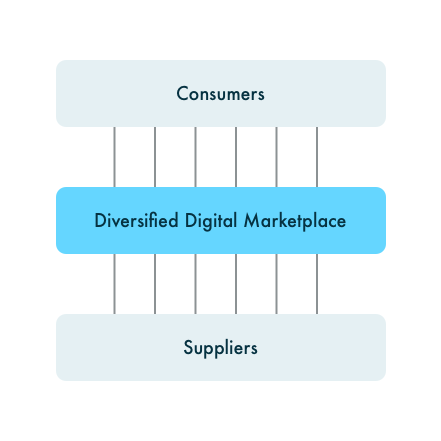
\includegraphics[scale=0.5]{figures/diversified.png}
\end{center}
\caption[Diversified Marketplaces]{Diversified Marketplaces connect consumers and sellers transparently}
\label{diversified_marketplace}
\end{figure}

\subsection{Commodified Marketplaces}
Commodified Marketplaces, the focus of this paper, sell a specific service (or set of services) to consumers. Each service is commodified and priced independent of which supplier ultimately provides the service. For example, Uber gives you a price estimate based on the ride (the service) not the driver (the supplier). Commodified marketplaces like Uber and Instacart offer services to consumers without the complication of who or how. These marketplaces are opaque by design, streamlining the provision of the service and shielding consumers from the details. They also tend to focus on niche services in order to polish the user experience. For example, Wag commodified dog walks.
\begin{figure}[ht!]
\begin{center}
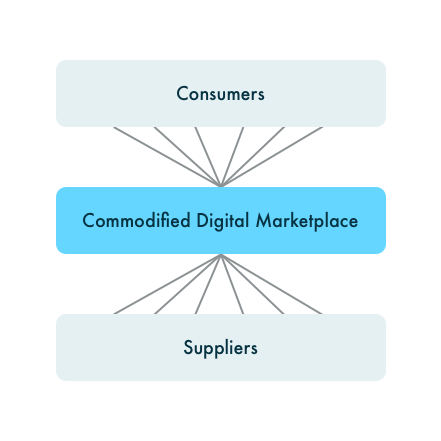
\includegraphics[scale=0.5]{figures/commodified.png}
\end{center}
\caption[Commodified Marketplaces]{Diversified Marketplaces connect consumers and sellers opaquely}
\label{commodified_marketplace}
\end{figure}  

\begin{table}
  \begin{center}
  \begin{tabular}{|l|p{4cm}|c|c|}
  \hline
  {\sc Name}  &  {\sc Description} & {\sc Classification} & {\sc URL} \\
  \hline
  Amazon          & Online seller of almost anything & Diversified & \url{https://amazon.com} \\
  \hline
  Uber      & On-demand rides & Commodified & \url{https://uber.com} \\
  \hline
  Instacart    & Grocery delivery & Commodified & \url{https://instacart.com} \\
  \hline
  Wag!  & Pet services & Commodified & \url{https://wagwalking.com} \\
  \hline
  DoorDash  & Food delivery & Commodified & \url{https://doordash.com} \\
  \hline
  lugg  & Move anything with the tap of a button & Commodified & \url{https://lugg.com} \\
  \hline
  Thumbtack  & Find a local pro for pretty much anything & Diversified & \url{https://thumbtack.com} \\
  \hline
  \end{tabular}
  \end{center}
  \caption{Examples of Digital Marketplaces}
  \label{digital_marketplaces}
  \end{table}

\section{Changing definition of work and the gig economy}
The nature of work is changing as our economy evolves. More and more people are employed in the gig economy, working flexible hours under the umbrella of some digital marketplace. Instead of working for a taxi company, drivers are providing rides through Uber. With this transition, service providers are reorganizing and the incentive structures must be re-evaluated. As a result of this reorganization, many workers are losing benefits and protections that were once considered essential, such as healthcare and severance.

\section{Power of a platform to organize economic activity}
The macroeconomic shift to the gig economy and the enormous value creation and provision from digital markeplaces highlight the power that these platforms have to organize economic activity and the wellbeing of millions (maybe billions) of people. These platforms are immensely powerful – they shape the very fabric of our economy. This is especially true in The United States, where  Services made up over 77\% of the economy in 2017 \citep{economyDistribution}.

\section{Research landscape}
Despite their significance and relevance, digital marketplaces are still a relatively new phenomenon, and much research remains underdeveloped. Successful digital marketplaces like Uber have created large teams of economists in an attempt to optimize their operations, but their inquiry is specific to their individual challenges. This paper is intended to provide a reductionist theory and some practical considerations that can be broadly applied to commodified digital marketplaces.